% =====================================================================
%  MẪU BÁO CÁO MÔN HỌC CHO SINH VIÊN - Nguyễn Tuấn Anh
%  Biên dịch bằng XeLaTeX (chạy 2-3 lần để cập nhật mục lục, trích dẫn).
%  Trên Overleaf: Menu > Compiler > XeLaTeX
%
%  Cấu trúc:
%    Bìa chính -> Bìa phụ -> Nhận xét của GV -> Lời cam đoan -> Lời cảm ơn
%    -> Mục lục -> Danh mục hình -> Danh mục bảng -> Danh mục từ viết tắt
%    -> Mở đầu -> Chương 1..3 -> Kết luận và hướng phát triển
%    -> Tài liệu tham khảo -> Phụ lục
%
%  SINH VIÊN CHỈ CẦN SỬA THÔNG TIN Ở MỤC "THÔNG TIN BÁO CÁO" BÊN DƯỚI.
% =====================================================================
\RequirePackage{fix-cm}   % cho phép cỡ chữ 13pt với phông toán mặc định
\documentclass[12pt,a4paper,oneside]{report}

% Cỡ chữ thân bài 13pt (giống bản Word)
\makeatletter
\renewcommand\normalsize{%
  \@setfontsize\normalsize{13pt}{15.6pt}%
  \abovedisplayskip 12pt plus3pt minus7pt
  \belowdisplayskip \abovedisplayskip
  \abovedisplayshortskip 0pt plus3pt
  \belowdisplayshortskip 6.5pt plus3.5pt minus3pt}
\normalsize
\makeatother

% ---------------- Trang giấy & phông chữ ----------------
% Lề theo quy định trình bày văn bản: trái 3cm, phải 2cm, trên 2cm, dưới 2,5cm
\usepackage[a4paper,left=3cm,right=2cm,top=2cm,bottom=2.5cm]{geometry}
\usepackage{fontspec}
\setmainfont{Times New Roman}
\usepackage[vietnamese]{babel}
\usepackage{setspace}
\setstretch{1.3}
\setlength{\parindent}{1cm}
\setlength{\parskip}{6pt}
\usepackage{indentfirst}

% ---------------- Gói hỗ trợ ----------------
\usepackage{amsmath,amssymb}
\usepackage{graphicx}
\graphicspath{{images/}}
\usepackage{float}
\usepackage{array}
\usepackage{longtable}
\usepackage{caption}
\captionsetup{labelsep=colon,font=normalsize,skip=6pt}
\usepackage{titlesec}
\usepackage{titletoc}
\usepackage{enumitem}
\setlist{nosep,leftmargin=1.5cm}
\usepackage{cite}          % gộp trích dẫn: [4-6], [2, 4-6]
\usepackage{fancyhdr}
\usepackage{tikz}          % khung viền trang bìa
\usepackage[hidelinks,unicode,bookmarksnumbered,bookmarksopen]{hyperref}
\usepackage{bookmark}

% ---------------- THÔNG TIN BÁO CÁO (sinh viên sửa tại đây) ----------------
\newcommand{\TenTruong}{TRƯỜNG ĐẠI HỌC CÔNG NGHỆ THÔNG TIN VÀ TRUYỀN THÔNG}
\newcommand{\TenKhoa}{KHOA CÔNG NGHỆ THÔNG TIN}
\newcommand{\TenBoMon}{BỘ MÔN KHOA HỌC MÁY TÍNH}
\newcommand{\LoaiBaoCao}{BÁO CÁO MÔN HỌC}
\newcommand{\TenHocPhan}{HỌC MÁY}
\newcommand{\TenDeTai}{ỨNG DỤNG HỌC MÁY TRONG DỰ ĐOÁN\\[4pt] KẾT QUẢ HỌC TẬP CỦA SINH VIÊN}
\newcommand{\TenDeTaiPDF}{Ứng dụng học máy trong dự đoán kết quả học tập của sinh viên}
\newcommand{\GiangVien}{TS. Nguyễn Văn A}
\newcommand{\SinhVien}{Nguyễn Văn B}
\newcommand{\MaSinhVien}{DTC22xxxxxxxx}
\newcommand{\Lop}{KHMT K22A}
\newcommand{\NoiNam}{Thái Nguyên, năm 2026}

\hypersetup{
  pdftitle={\TenDeTaiPDF},
  pdfauthor={\SinhVien},
  pdfsubject={Báo cáo môn học Học máy},
  pdfkeywords={học máy, báo cáo môn học}
}

% ---------------- Đánh số trang (chân trang, giữa) ----------------
\pagestyle{fancy}
\fancyhf{}
\fancyfoot[C]{\thepage}
\renewcommand{\headrulewidth}{0pt}
\fancypagestyle{plain}{\fancyhf{}\fancyfoot[C]{\thepage}\renewcommand{\headrulewidth}{0pt}}

% ---------------- Tên gọi tiếng Việt ----------------
\addto\captionsvietnamese{%
  \renewcommand{\contentsname}{MỤC LỤC}%
  \renewcommand{\listfigurename}{DANH MỤC HÌNH ẢNH}%
  \renewcommand{\listtablename}{DANH MỤC BẢNG}%
  \renewcommand{\bibname}{TÀI LIỆU THAM KHẢO}%
  \renewcommand{\figurename}{Hình}%
  \renewcommand{\tablename}{Bảng}%
  \renewcommand{\chaptername}{Chương}%
  \renewcommand{\appendixname}{Phụ lục}%
}

% Hình và bảng đánh số theo chương (Hình 1.1, Bảng 1.1)
\renewcommand{\thefigure}{\thechapter.\arabic{figure}}
\renewcommand{\thetable}{\thechapter.\arabic{table}}

% Danh mục hình/bảng: ghi "Hình 1.1." / "Bảng 1.1." trước tên
\titlecontents{figure}[0pt]{}
  {\figurename~\thecontentslabel.\enspace}{}{\titlerule*[0.6pc]{.}\contentspage}
\titlecontents{table}[0pt]{}
  {\tablename~\thecontentslabel.\enspace}{}{\titlerule*[0.6pc]{.}\contentspage}

% ---------------- Định dạng tiêu đề ----------------
% Chương: "CHƯƠNG 1" dòng trên, tên chương in hoa dòng dưới - 14pt, đậm, căn giữa
\titleformat{\chapter}[display]
  {\centering\bfseries\fontsize{14}{18}\selectfont}
  {\MakeUppercase{\chaptername}~\thechapter}{4pt}{\MakeUppercase}
\titlespacing*{\chapter}{0pt}{0pt}{18pt}
% Chương không đánh số (Mở đầu, Lời cam đoan, ...)
\titleformat{name=\chapter,numberless}[block]
  {\centering\bfseries\fontsize{14}{18}\selectfont}{}{0pt}{\MakeUppercase}
\titlespacing*{name=\chapter,numberless}{0pt}{0pt}{18pt}
% Mục cấp 2: "1.1. Giới thiệu" - 14pt, đậm
\titleformat{\section}
  {\bfseries\fontsize{14}{18}\selectfont}{\thesection.}{0.5em}{}
\titlespacing*{\section}{0pt}{12pt}{6pt}
% Mục cấp 3: "1.4.1. Mục 1" - 13pt, đậm
\titleformat{\subsection}
  {\bfseries\fontsize{13}{17}\selectfont}{\thesubsection.}{0.5em}{}
\titlespacing*{\subsection}{0pt}{10pt}{6pt}
% Mục cấp 4: "1.4.1.1. ..." - 13pt, đậm nghiêng
\setcounter{secnumdepth}{3}
\titleformat{\subsubsection}
  {\bfseries\itshape\fontsize{13}{17}\selectfont}{\thesubsubsection.}{0.5em}{}
\titlespacing*{\subsubsection}{0pt}{8pt}{4pt}

% Mục lục: ghi "Chương 1." trước tên chương
\setcounter{tocdepth}{2}
\titlecontents{chapter}[0pt]{\addvspace{4pt}\bfseries}
  {\chaptername~\thecontentslabel.\enspace}{}{\titlerule*[0.6pc]{.}\contentspage}
\titlecontents{section}[1.5em]{}
  {\thecontentslabel.\enspace}{}{\titlerule*[0.6pc]{.}\contentspage}
\titlecontents{subsection}[3em]{}
  {\thecontentslabel.\enspace}{}{\titlerule*[0.6pc]{.}\contentspage}

% Chương không đánh số nhưng vẫn có trong mục lục và bookmark PDF
\newcommand{\unnumberedchapter}[1]{%
  \chapter*{#1}\phantomsection
  \addcontentsline{toc}{chapter}{\texorpdfstring{\MakeUppercase{#1}}{#1}}%
  \markboth{#1}{#1}}

% Bảng trống 3 cột làm mẫu
\newcolumntype{C}{>{\centering\arraybackslash}p{0.27\textwidth}}

\begin{document}

% =====================================================================
%  BÌA CHÍNH (không đánh số trang)
% =====================================================================
\begin{titlepage}
\begin{tikzpicture}[remember picture,overlay]
  \draw[line width=2pt]
    ([xshift=2.5cm,yshift=-1.5cm]current page.north west) rectangle
    ([xshift=-1.5cm,yshift=1.5cm]current page.south east);
  \draw[line width=0.6pt]
    ([xshift=2.65cm,yshift=-1.65cm]current page.north west) rectangle
    ([xshift=-1.65cm,yshift=1.65cm]current page.south east);
\end{tikzpicture}
\centering
\setstretch{1.2}
{\fontsize{13}{17}\selectfont \TenTruong\par}
{\fontsize{14}{18}\selectfont\bfseries \TenKhoa\par}
\vspace{2pt}
\rule{5cm}{0.8pt}\par

\vspace{3.5cm}
{\fontsize{24}{30}\selectfont\bfseries \LoaiBaoCao\par}
\vspace{6pt}
{\fontsize{18}{24}\selectfont\bfseries HỌC PHẦN: \TenHocPhan\par}

\vspace{2cm}
{\fontsize{14}{18}\selectfont\bfseries ĐỀ TÀI\par}
\vspace{6pt}
{\fontsize{18}{26}\selectfont\bfseries \TenDeTai\par}

\vspace{2.5cm}
{\fontsize{14}{20}\selectfont
\begin{tabular}{@{}l@{\hspace{1em}}l@{}}
  Giảng viên hướng dẫn: & \textbf{\GiangVien} \\
  Sinh viên thực hiện:  & \textbf{\SinhVien} \\
  Mã sinh viên:         & \MaSinhVien \\
  Lớp:                  & \Lop \\
\end{tabular}\par}

\vfill
{\fontsize{14}{18}\selectfont\bfseries \NoiNam\par}
\end{titlepage}

% =====================================================================
%  PHẦN ĐẦU: đánh số trang La Mã (i, ii, iii, ...)
% =====================================================================
\pagenumbering{roman}
\setcounter{page}{1}

% ---------------- BÌA PHỤ ----------------
\begin{titlepage}
\centering
\setstretch{1.2}
{\fontsize{13}{17}\selectfont \TenTruong\par}
{\fontsize{14}{18}\selectfont\bfseries \TenKhoa\par}
\vspace{2pt}
\rule{5cm}{0.8pt}\par

\vspace{3.5cm}
{\fontsize{14}{18}\selectfont\bfseries \SinhVien\par}

\vspace{2cm}
{\fontsize{18}{26}\selectfont\bfseries \TenDeTai\par}

\vspace{1.5cm}
{\fontsize{16}{20}\selectfont\bfseries \LoaiBaoCao{} \TenHocPhan\par}
\vspace{4pt}
{\fontsize{14}{18}\selectfont Chuyên ngành: Khoa học máy tính\par}

\vspace{2.5cm}
{\fontsize{14}{20}\selectfont
\begin{tabular}{@{}l@{\hspace{1em}}l@{}}
  Giảng viên hướng dẫn: & \textbf{\GiangVien} \\
\end{tabular}\par}

\vfill
{\fontsize{14}{18}\selectfont\bfseries \NoiNam\par}
\end{titlepage}
\setcounter{page}{2}

% ---------------- NHẬN XÉT CỦA GIẢNG VIÊN ----------------
\unnumberedchapter{Nhận xét của giảng viên}

\noindent\textbf{Họ và tên sinh viên:} \SinhVien\hfill\textbf{Mã SV:} \MaSinhVien

\noindent\textbf{Đề tài:} \TenDeTaiPDF

\vspace{6pt}
\noindent\textbf{Nhận xét:}

\noindent
\foreach \i in {1,...,12}{\makebox[\linewidth]{\dotfill}\\[4pt]}

\vspace{6pt}
\noindent\textbf{Điểm đánh giá:} \dotfill\quad (Bằng chữ: \dotfill)

\vspace{1cm}
\hfill
\begin{minipage}{0.5\textwidth}
  \centering
  Thái Nguyên, ngày \dots\ tháng \dots\ năm 20\dots\\
  \textbf{Giảng viên}\\
  \textit{(Ký và ghi rõ họ tên)}
\end{minipage}

% ---------------- LỜI CAM ĐOAN ----------------
\unnumberedchapter{Lời cam đoan}

Em xin cam đoan báo cáo môn học \textbf{\TenHocPhan} với đề tài
``\TenDeTaiPDF'' là kết quả học tập và tìm hiểu của riêng em dưới sự hướng
dẫn của \GiangVien. Các nội dung, số liệu và kết quả trình bày trong báo
cáo là trung thực, chưa từng được công bố trong bất kỳ công trình nào khác.

Những phần tham khảo từ các tài liệu, công trình của tác giả khác đều được
trích dẫn rõ ràng và liệt kê đầy đủ trong mục Tài liệu tham khảo. Nếu phát
hiện có bất kỳ sự gian lận nào, em xin hoàn toàn chịu trách nhiệm trước
giảng viên và Nhà trường.

\vspace{1cm}
\hfill
\begin{minipage}{0.5\textwidth}
  \centering
  Thái Nguyên, ngày \dots\ tháng \dots\ năm 20\dots\\
  \textbf{Sinh viên thực hiện}\\
  \textit{(Ký và ghi rõ họ tên)}\\[2cm]
  \SinhVien
\end{minipage}

% ---------------- LỜI CẢM ƠN ----------------
\unnumberedchapter{Lời cảm ơn}

Em xin chân thành cảm ơn các thầy cô giáo trong \TenKhoa{} --
\TenTruong{} đã trang bị cho em những kiến thức nền tảng trong suốt quá
trình học tập.

Đặc biệt, em xin gửi lời cảm ơn sâu sắc tới \GiangVien{} đã tận tình hướng
dẫn, góp ý để em hoàn thành báo cáo này.

Do thời gian và kiến thức còn hạn chế, báo cáo không tránh khỏi những
thiếu sót. Em rất mong nhận được ý kiến đóng góp của thầy cô để báo cáo
được hoàn thiện hơn.

\vspace{6pt}
\hfill\textit{Em xin chân thành cảm ơn!}

% ---------------- MỤC LỤC, DANH MỤC HÌNH, BẢNG ----------------
\clearpage
\phantomsection\addcontentsline{toc}{chapter}{MỤC LỤC}
\tableofcontents
\clearpage
\phantomsection\addcontentsline{toc}{chapter}{DANH MỤC HÌNH ẢNH}
\listoffigures
\clearpage
\phantomsection\addcontentsline{toc}{chapter}{DANH MỤC BẢNG}
\listoftables

% ---------------- DANH MỤC TỪ VIẾT TẮT ----------------
\unnumberedchapter{Danh mục từ viết tắt}

\begin{center}
\renewcommand{\arraystretch}{1.3}
\begin{longtable}{|>{\centering\arraybackslash}p{0.07\textwidth}|
                  >{\raggedright\arraybackslash}p{0.2\textwidth}|
                  >{\raggedright\arraybackslash}p{0.6\textwidth}|}
  \hline
  \textbf{STT} & \textbf{Viết tắt} & \textbf{Ý nghĩa} \\ \hline
  \endhead
  1 & CMD     & Command Prompt -- cửa sổ dòng lệnh của Windows \\ \hline
  2 & KNN     & K-Nearest Neighbors -- K láng giềng gần nhất \\ \hline
  3 & SVM     & Support Vector Machine -- Máy véc-tơ hỗ trợ \\ \hline
  4 & XGBoost & Extreme Gradient Boosting \\ \hline
  5 & ICTU    & Trường Đại học Công nghệ Thông tin và Truyền thông \\ \hline
\end{longtable}
\end{center}

% =====================================================================
%  PHẦN NỘI DUNG: đánh số trang Ả Rập (1, 2, 3, ...)
% =====================================================================
\clearpage
\pagenumbering{arabic}
\setcounter{page}{1}

% =====================================================================
%  MỞ ĐẦU
% =====================================================================
\unnumberedchapter{Mở đầu}

Trong một báo cáo khoa học, báo cáo môn học hay báo cáo nghiên cứu, phần
Lời mở đầu (hoặc Mở đầu) thường được viết ngắn gọn, súc tích và cần đảm
bảo các nội dung sau:

\textbf{1. Giới thiệu bối cảnh và lý do chọn đề tài}

Nêu tình hình thực tiễn, lý do tại sao vấn đề được quan tâm.

Giải thích tầm quan trọng, ý nghĩa khoa học hoặc ý nghĩa thực tiễn.

\textbf{2. Mục tiêu và nhiệm vụ nghiên cứu}

Trình bày rõ báo cáo nhằm đạt được mục tiêu gì.

Nêu các nhiệm vụ chính mà nhóm/cá nhân thực hiện.

\textbf{3. Phạm vi và đối tượng nghiên cứu}

Xác định rõ phạm vi ứng dụng, dữ liệu, mô hình hay hệ thống được nghiên cứu.

Giới hạn nội dung để tránh bị lan man.

\textbf{4. Phương pháp tiếp cận (ngắn gọn)}

Có thể đề cập sơ lược phương pháp nghiên cứu, công cụ hoặc cách tiếp cận.

\textbf{5. Kết cấu báo cáo (nếu cần)}

Giới thiệu sơ bộ các phần nội dung chính trong báo cáo (ví dụ: Chương 1
-- Cơ sở lý thuyết, Chương 2 -- Phân tích dữ liệu, Chương 3 -- Kết quả
và thảo luận\dots).

% =====================================================================
%  CHƯƠNG 1
% =====================================================================
\chapter{Tổng quan về học máy}

\section{Giới thiệu}

\section{Giới thiệu cái gì đó}

Nội dung trình bày. Khi tham chiếu hình, bảng trong văn bản nên dùng
\verb|\ref|, ví dụ: Hình~\ref{fig:run-1}, Hình~\ref{fig:cmd-1},
Bảng~\ref{tab:can-bo-lop}.

\begin{figure}[H]
  \centering
  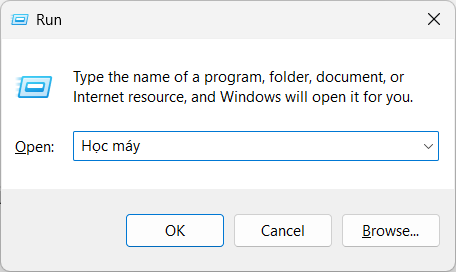
\includegraphics[width=8.84cm]{image1.png}
  \caption{Cửa sổ chạy chương trình RUN}
  \label{fig:run-1}
\end{figure}

\begin{figure}[H]
  \centering
  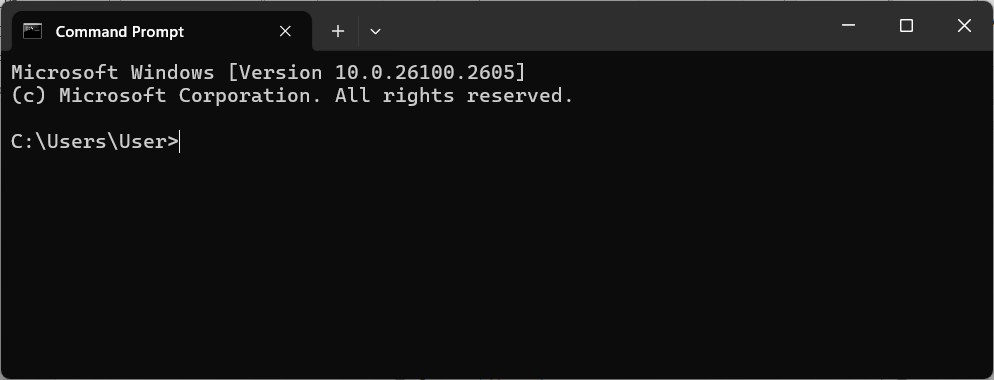
\includegraphics[width=11.12cm]{image2.png}
  \caption{Cửa sổ CMD}
  \label{fig:cmd-1}
\end{figure}

\begin{table}[H]
  \centering
  \caption{Danh sách cán bộ lớp}
  \label{tab:can-bo-lop}
  \begin{tabular}{|C|C|C|}
    \hline
     &  &  \\ \hline
     &  &  \\ \hline
     &  &  \\ \hline
  \end{tabular}
\end{table}

\begin{table}[H]
  \centering
  \caption{Danh sách sinh viên}
  \label{tab:sinh-vien}
  \begin{tabular}{|C|C|C|}
    \hline
     &  &  \\ \hline
     &  &  \\ \hline
  \end{tabular}
\end{table}

\begin{table}[H]
  \centering
  \caption{Danh sách sinh viên K20}
  \label{tab:k20}
  \begin{tabular}{|C|C|C|}
    \hline
     &  &  \\ \hline
     &  &  \\ \hline
  \end{tabular}
\end{table}

\begin{table}[H]
  \centering
  \caption{Danh sách sinh viên K21}
  \label{tab:k21}
  \begin{tabular}{|C|C|C|}
    \hline
     &  &  \\ \hline
     &  &  \\ \hline
  \end{tabular}
\end{table}

\begin{table}[H]
  \centering
  \caption{Danh sách sinh viên K22}
  \label{tab:k22}
  \begin{tabular}{|C|C|C|}
    \hline
     &  &  \\ \hline
     &  &  \\ \hline
  \end{tabular}
\end{table}

\begin{table}[H]
  \centering
  \caption{Danh sách sinh viên K23}
  \label{tab:k23}
  \begin{tabular}{|C|C|C|}
    \hline
     &  &  \\ \hline
     &  &  \\ \hline
  \end{tabular}
\end{table}

\section{Bài toán dự đoán điểm sinh viên}

Nghiên cứu sử dụng các mô hình học máy (Logistic Regression, KNN,
Decision Tree, Random Forest, SVM, XGBoost, CatBoost) để dự đoán tình
trạng tốt nghiệp đúng hạn của sinh viên ngành Ngân hàng (2010--2020).
Kết quả cho thấy Random Forest là mô hình tối ưu, với các thuộc tính như
thông tin học vụ và điểm trung bình học kỳ 1--4 ảnh hưởng mạnh đến khả
năng tốt nghiệp. Nghiên cứu đề xuất giải pháp giúp nâng cao tỷ lệ tốt
nghiệp của sinh viên \cite{hai2017,thuan2022,thuy2023}.

Nghiên cứu áp dụng học máy để dự đoán điểm thi cuối kỳ, tập trung xử lý
dữ liệu mất cân bằng. Phương pháp đạt hiệu suất cao nhất với Precision
43,70\%, Recall 45,1\% và F1-score 44,04\% \cite{lananh,hai2017,thuan2022,thuy2023}.

Theo công trình của Nguyễn Tuấn Anh \cite{alquraishi2021,tuananh2024}

\section{Một số bài toán điển hình}

\subsection{Mục 1}

\subsection{Mục 2}

\subsection{Mục 3}

\section{Kết luận chương 1}

% =====================================================================
%  CHƯƠNG 2
% =====================================================================
\chapter{Một số kỹ thuật phân cụm}

\section{Giới thiệu}

\begin{figure}[H]
  \centering
  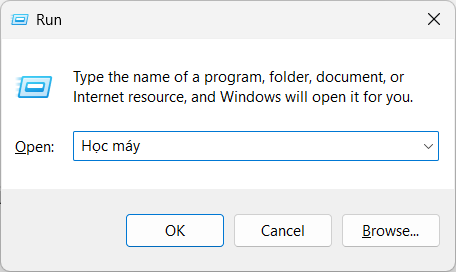
\includegraphics[width=8.84cm]{image1.png}
  \caption{Cửa sổ chạy chương trình RUN}
  \label{fig:run-2}
\end{figure}

\begin{figure}[H]
  \centering
  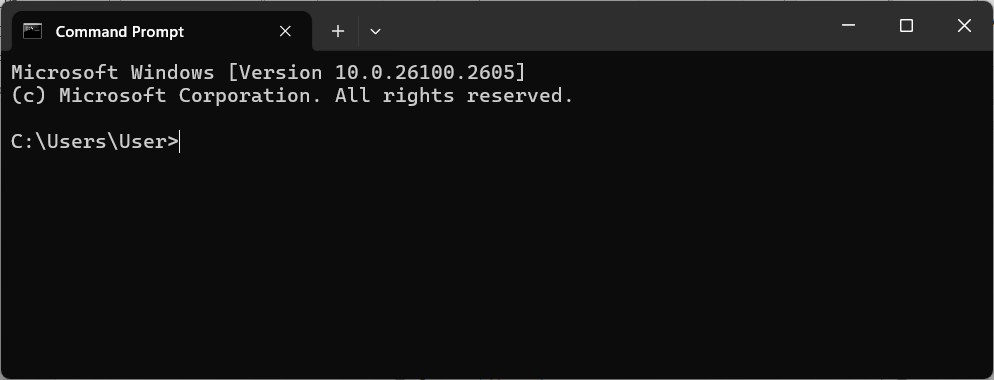
\includegraphics[width=11.12cm]{image2.png}
  \caption{Cửa sổ CMD}
  \label{fig:cmd-2}
\end{figure}

\section{Một số bài toán điển hình}

\subsection{Mục 1}

\subsection{Mục 2}

\subsection{Mục 3}

\section{Kết luận chương 2}

% =====================================================================
%  CHƯƠNG 3
% =====================================================================
\chapter{Thử nghiệm và đánh giá}

\section{Giới thiệu}

\begin{figure}[H]
  \centering
  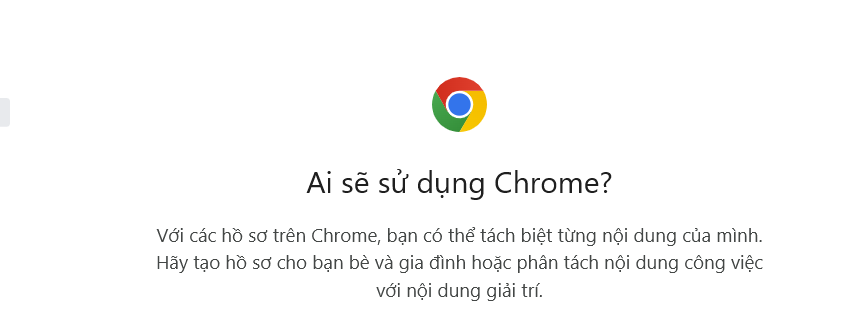
\includegraphics[width=\textwidth]{image3.png}
  \caption{Giao diện Chrome}
  \label{fig:chrome}
\end{figure}

\section{Một số bài toán điển hình}

\subsection{Mục 1}

\subsection{Mục 2}

\subsection{Mục 3}

\section{Phân tích và đánh giá}

\section{Kết luận chương 3}

% =====================================================================
%  KẾT LUẬN VÀ HƯỚNG PHÁT TRIỂN
% =====================================================================
\unnumberedchapter{Kết luận và hướng phát triển}

\textbf{1. Kết quả đạt được}

Tóm tắt các kết quả chính mà báo cáo đã đạt được so với mục tiêu đặt ra
ở phần Mở đầu.

\textbf{2. Hạn chế}

Nêu những điểm còn hạn chế của báo cáo (dữ liệu, mô hình, thời gian\dots).

\textbf{3. Hướng phát triển}

Đề xuất các hướng nghiên cứu, cải tiến tiếp theo.

% =====================================================================
%  TÀI LIỆU THAM KHẢO
% =====================================================================
\clearpage
\phantomsection
\addcontentsline{toc}{chapter}{TÀI LIỆU THAM KHẢO}
\begin{thebibliography}{9}

\bibitem{alquraishi2021}
Mohammed AlQuraishi (2021), ``Machine learning in protein structure
prediction'', \textit{Current opinion in chemical biology}. Tập 65, trang: 1--8.

\bibitem{lananh}
Nguyễn Thị Lan Anh, ``Cải thiện kết quả dự đoán điểm thi của sinh viên
bằng Máy học với sự hỗ trợ của R''.

\bibitem{tuananh2024}
Nguyễn Tuấn Anh (2024), ``Ứng dụng mô hình học máy vào trong dự đoán kết
quả học tập của sinh viên tại ICTU'', \textit{Tạp chí Khoa học và Công nghệ ĐHTN}.

\bibitem{hai2017}
Trương Thị Hải, Nguyễn Thái Nghe và Huỳnh Xuân Hiệp (2017), ``Giải pháp
hỗ trợ sinh viên lập kế hoạch học tập dựa trên tiếp cận tập thô'',
\textit{PROCEEDING of Publishing House for Science Technology}.

\bibitem{thuan2022}
Trần Bá Thuấn (2022), ``Ứng dụng machine learning dự báo sinh viên diện
cảnh báo học tập tại trường đại học kinh tế huế'', \textit{Tạp chí Khoa
học Quản lý và Kinh tế, Trường Đại học Kinh Tế, Đại học Huế}. (21).

\bibitem{thuy2023}
Nguyễn Văn Thủy (2023), ``Sử dụng các mô hình Machine Learning dự đoán
tình trạng sinh viên tốt nghiệp đúng hạn'', \textit{Tạp chí Khoa học Đào
tạo Ngân hàng}. Tập 225(8), trang: 52--64.

\end{thebibliography}

% =====================================================================
%  PHỤ LỤC
% =====================================================================
\clearpage
\phantomsection
\addcontentsline{toc}{chapter}{PHỤ LỤC}
\begin{center}
  {\bfseries\fontsize{14}{18}\selectfont PHỤ LỤC\par}
\end{center}
\vspace{12pt}

\noindent\textbf{Phụ lục A. Mã nguồn chương trình}

Đưa mã nguồn chính, đường dẫn kho mã (GitHub, Google Drive\dots) hoặc
notebook đã sử dụng trong báo cáo.

\noindent\textbf{Phụ lục B. Dữ liệu và kết quả bổ sung}

Mô tả bộ dữ liệu, các bảng kết quả chi tiết hoặc hình ảnh bổ sung không
đưa vào phần nội dung chính.

\end{document}
